\begin{frame}
	\begin{center}
		\Huge Minigames
	\end{center}
\end{frame}
	
\begin{frame}
	\frametitle{Ziele}
	\begin{itemize}
		\item Erhalten von Items, zur Nutzung im Kampf
		\item Abwechslung gegenüber den Kämpfen
	\end{itemize}
\end{frame}

\begin{frame}
	\frametitle{Allgemein}
	\begin{itemize}
		\item ein Minigame pro Fachschaft
		\item drei Level, progressiv schwerer
		\begin{itemize}
			\item Level 1: Einführung
			\item Level 2: \glqq standard\grqq-Schwierigkeit
			\item Level 3: Herausforderung
		\end{itemize}
		\item Item als Belohnung, der Schwierigkeit entsprechend
		\item jederzeit Spielbar
	\end{itemize}
\end{frame}

\begin{frame}
	\frametitle{Informatik}
	\begin{minipage}[l]{0.40\textwidth}
		\begin{itemize}
			\item Konzept: Vervollständigen von Schaltkreisen
			\item Level: unterschiedlich viele fehlende Gatter und Antwortmöglichkeiten
		\end{itemize}
	\end{minipage}
	\hfill
	\begin{minipage}[r]{0.55\textwidth}
		\centering
		\begin{figure}
			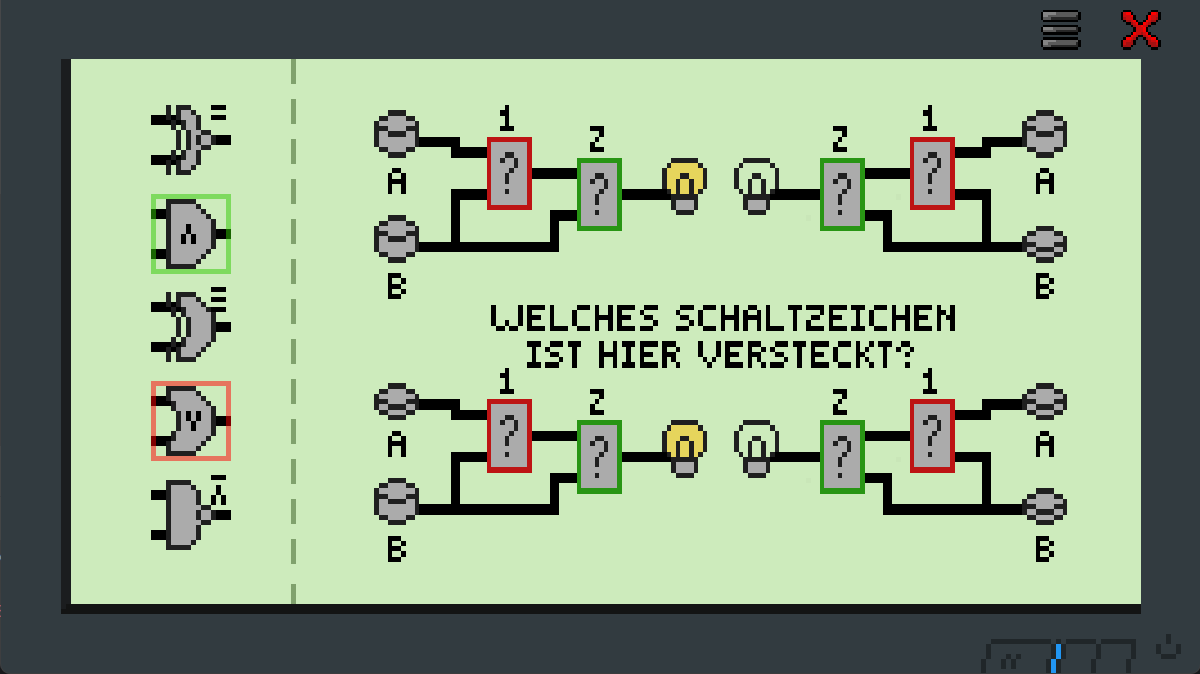
\includegraphics[width=\textwidth]{bilder/MinispielInformatik.png}
			\caption{Beispiel Informatik-Minigame (Bildschirmfoto des Projektes)}
		\end{figure}
	\end{minipage}
\end{frame}

\begin{frame}
	\frametitle{Informatik}
	Idee:
	\begin{itemize}
		\item Vervollständigen eines Schaltkreises
		\item Verhalten gegeben
		\item Antwortmöglichkeiten gegeben
	\end{itemize}
\end{frame}

\begin{frame}
	\frametitle{Mathematik}
\end{frame}

\begin{frame}
	\frametitle{Das Chemie-Minigame}
\begin{minipage}[l]{0.40\textwidth}
	\begin{itemize}
		\item Konzept: Watersort-Puzzle
		\item Level: untersch. viele Farben und Gläser
		\end{itemize}
\end{minipage}
\begin{minipage}[r]{0.55\textwidth}
	\centering
	\begin{figure}
	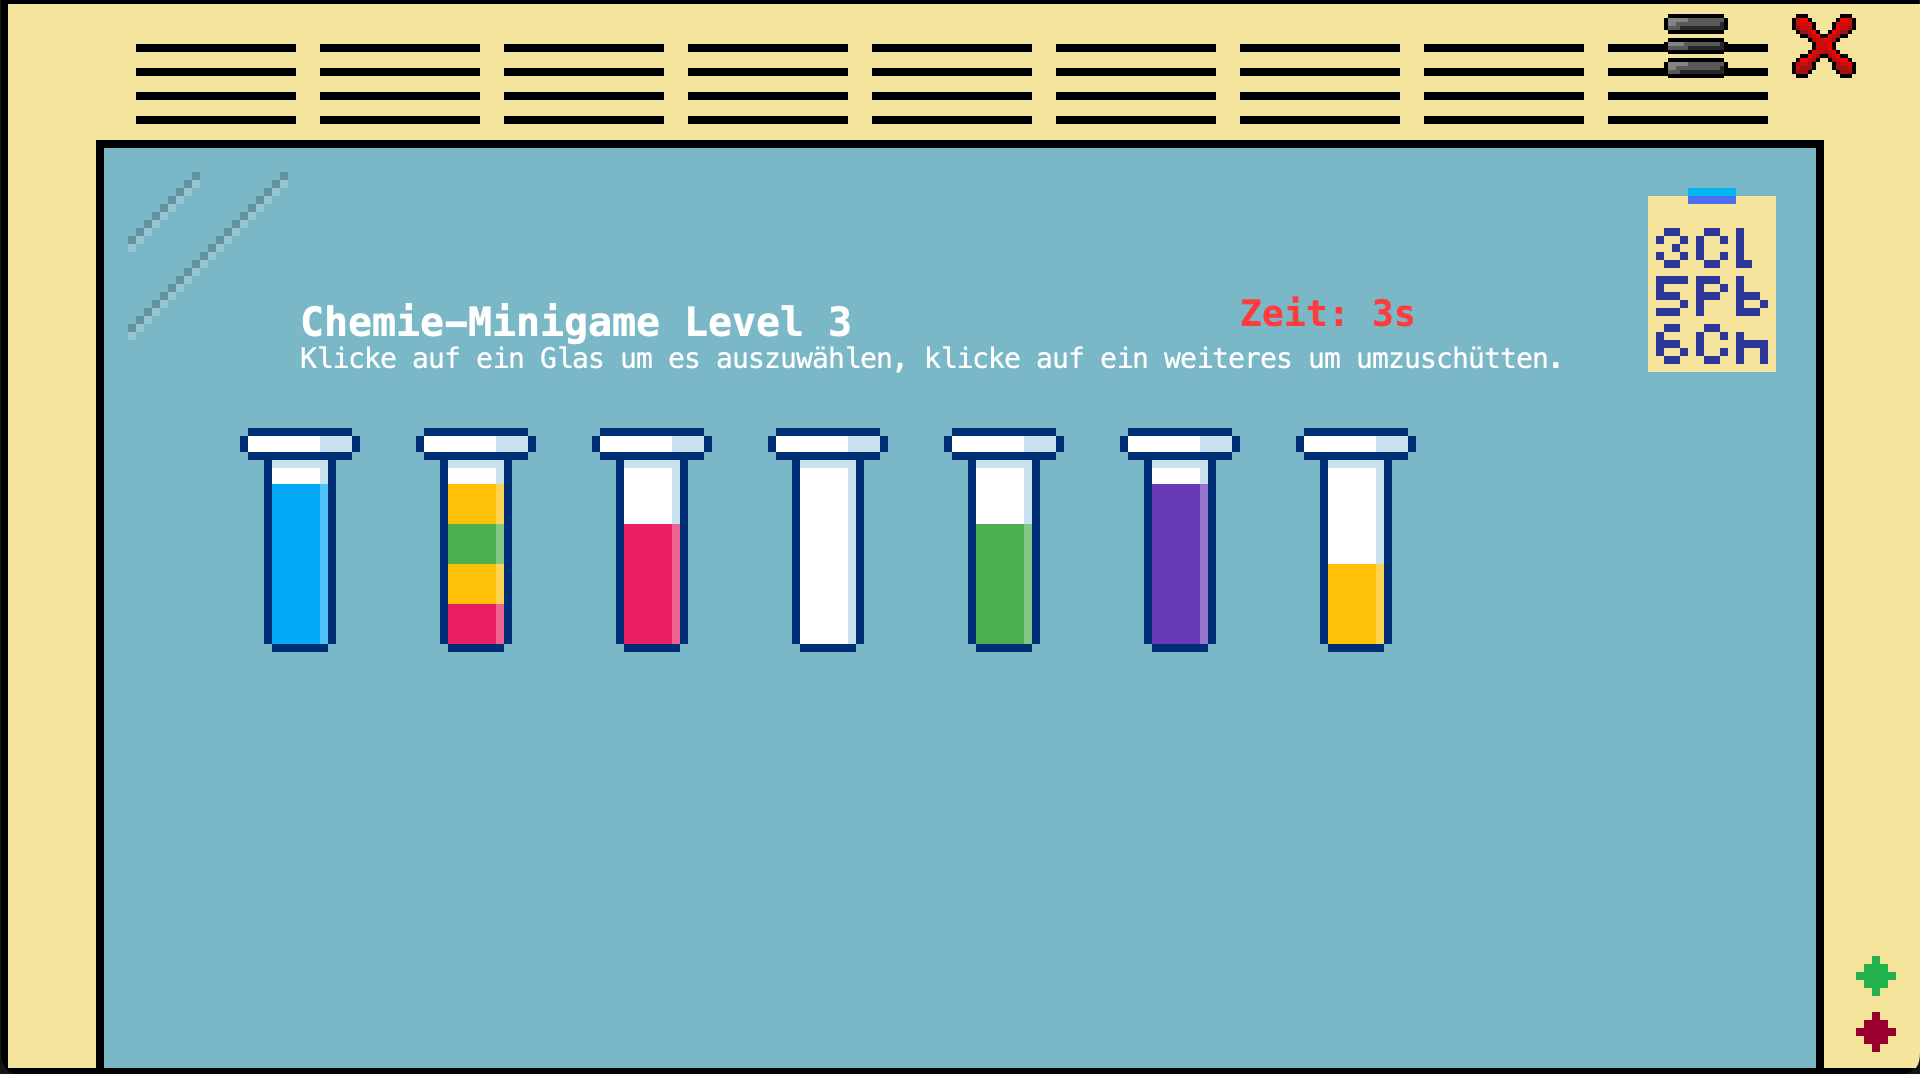
\includegraphics[width=\textwidth]{../dokumentation/bilder/BeispielChemie.png}
	\caption{Beispiel Chemie-Minigame}
	\end{figure}
\end{minipage}
\end{frame}

\begin{frame}
	\frametitle{Spielmechanik}
	\begin{figure}
		\centering
		\begin{minipage}[l]{0.3\textwidth}
			\centering
			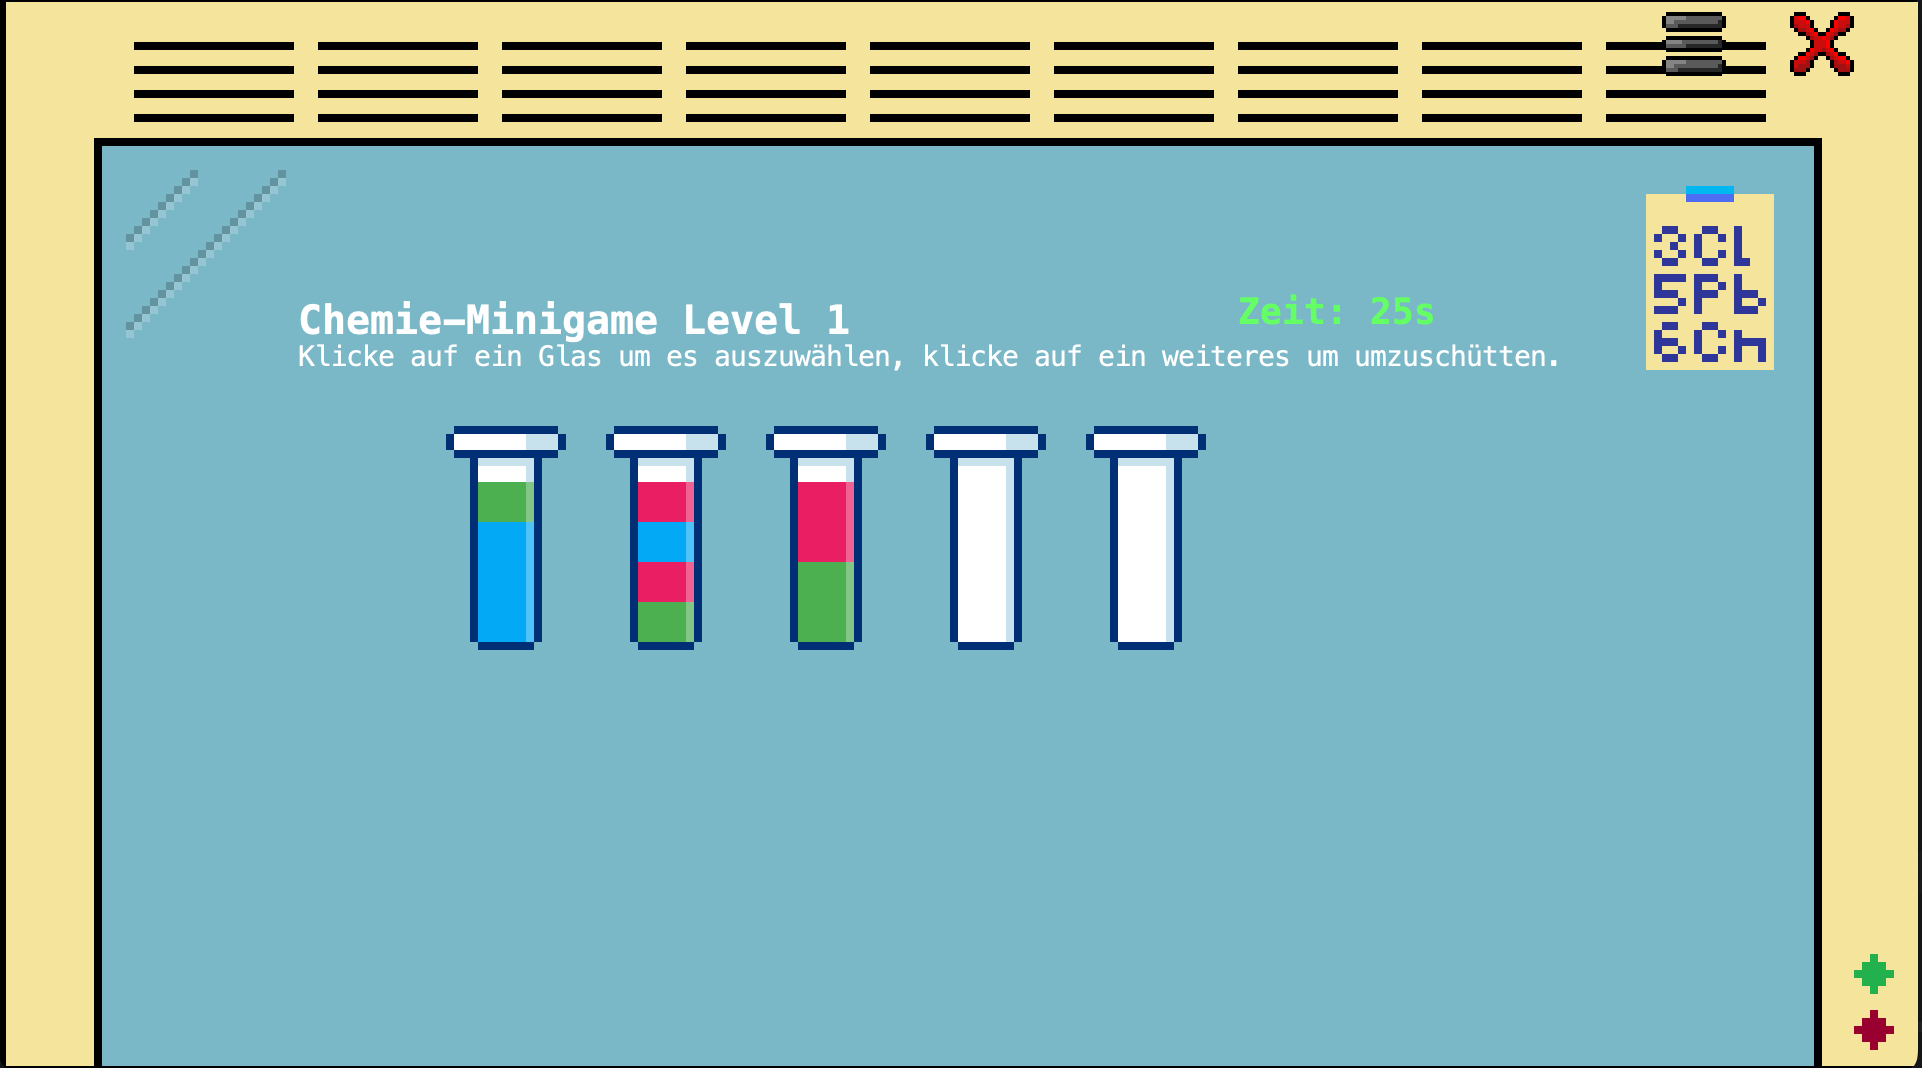
\includegraphics[width=\linewidth]{../präsi/bilder/ChemieLevelStart.png}
			\caption{Levelstart}
		\end{minipage}
		\hfill
		$\Rightarrow$
		\hfill
		\begin{minipage}[l]{0.3\textwidth}
			\centering
			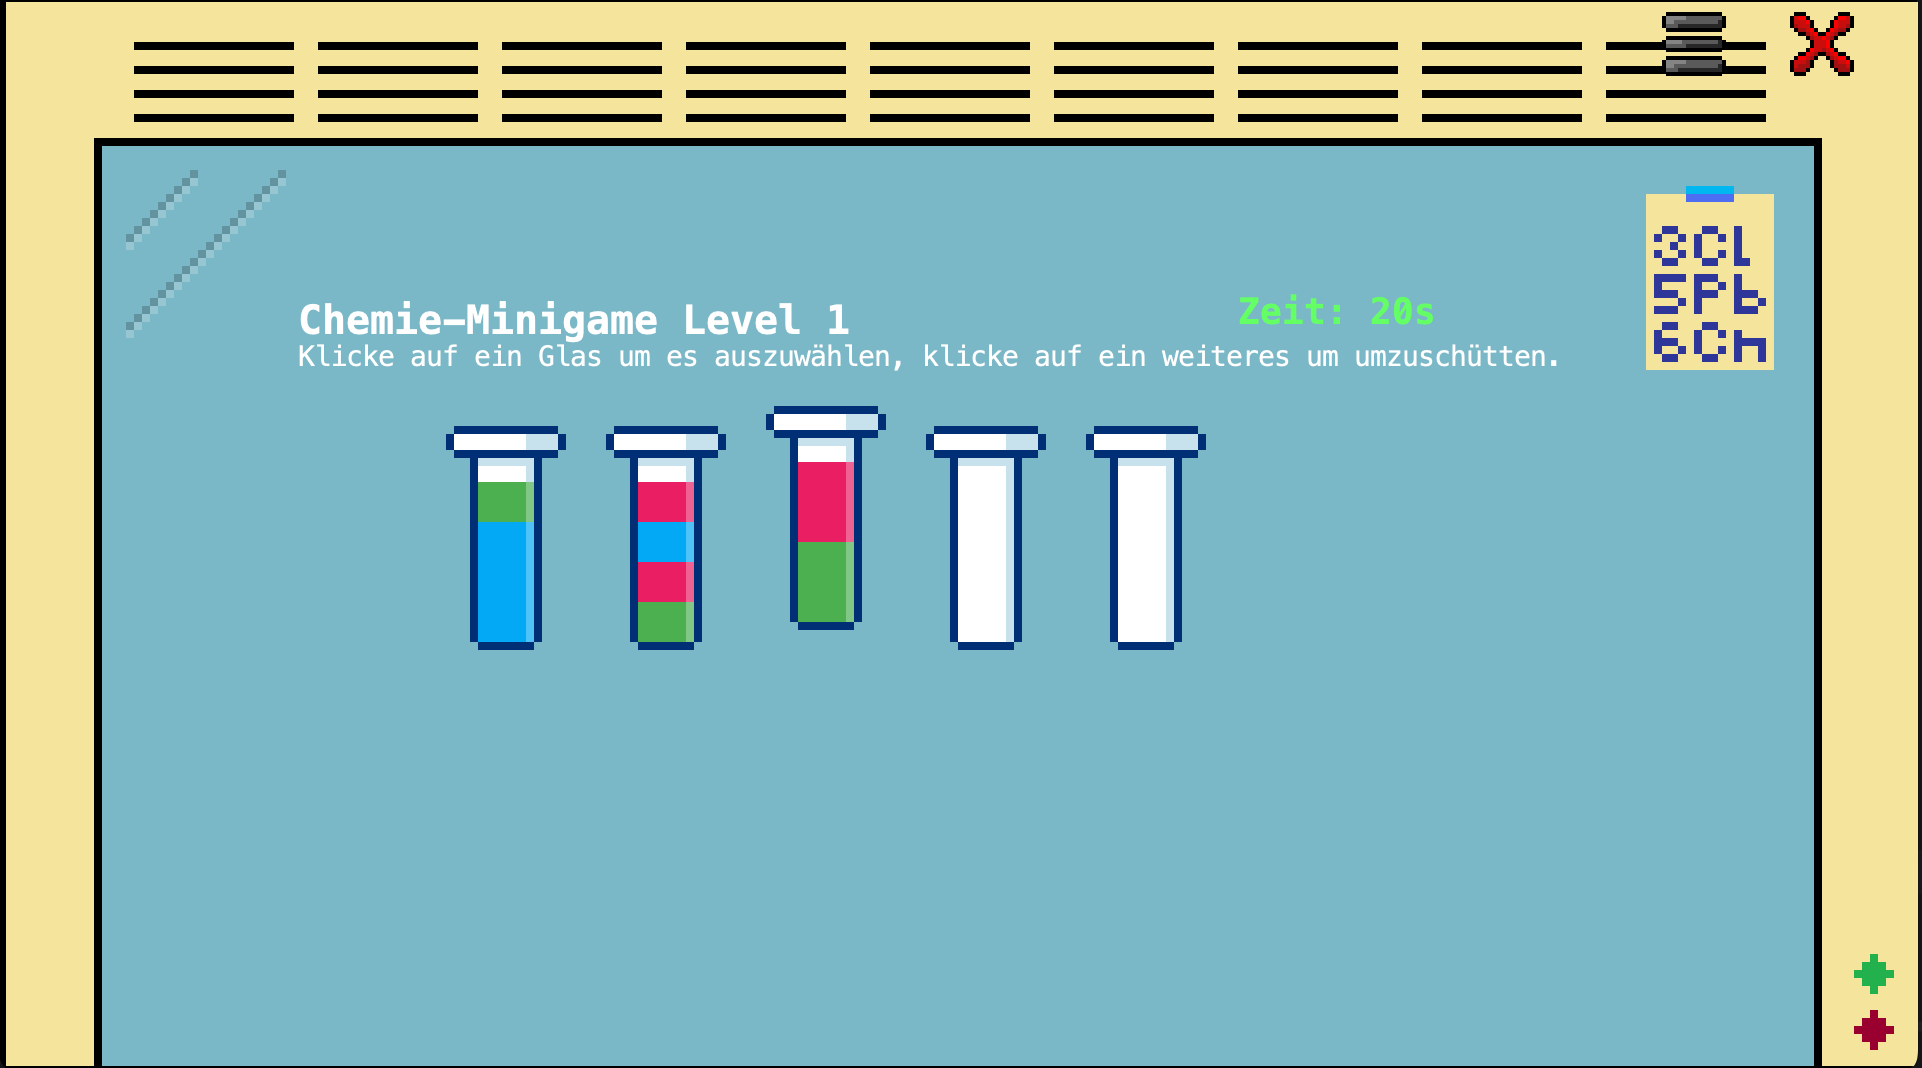
\includegraphics[width=\linewidth]{../präsi/bilder/ChemieGlasAuswahl.png}
			\caption{Glas auswählen}
		\end{minipage}
		\hfill
		$\Rightarrow$
		\hfill
		\begin{minipage}[l]{0.3\textwidth}
			\centering
			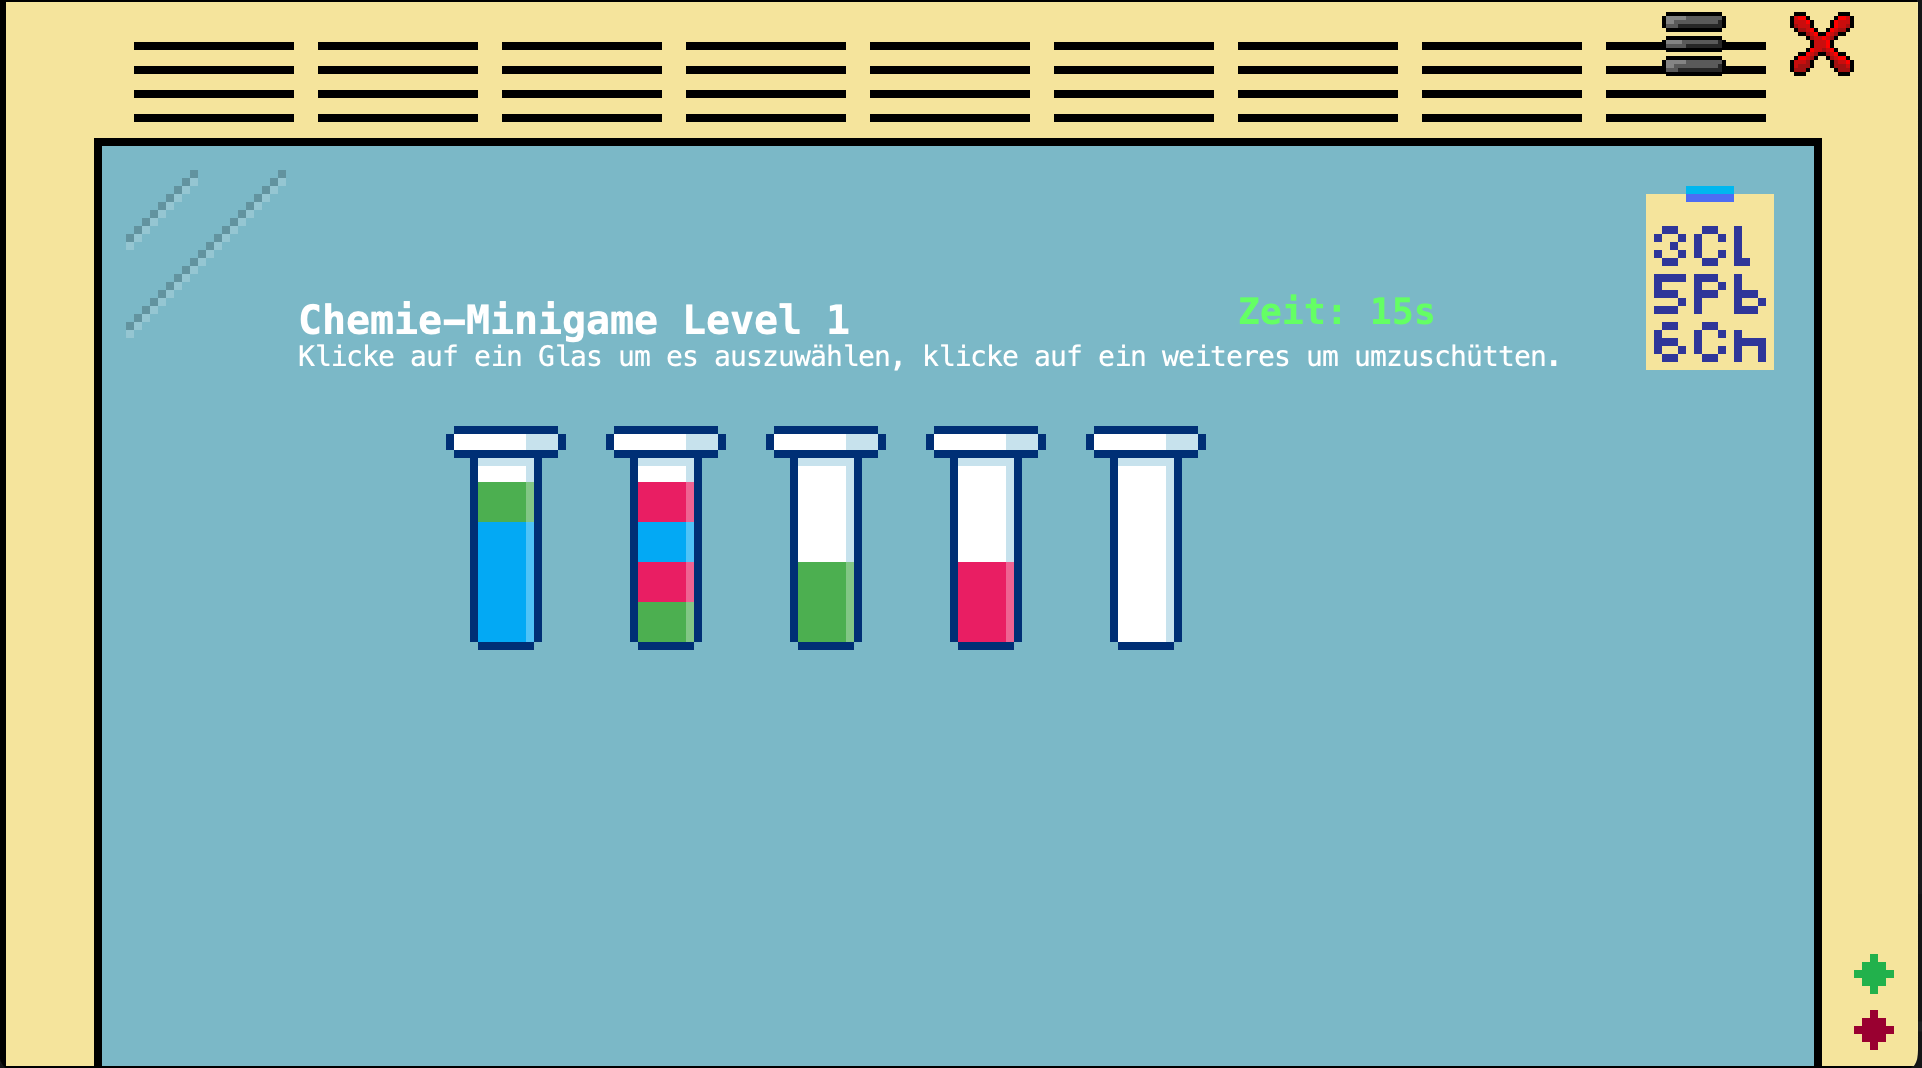
\includegraphics[width=\linewidth]{../präsi/bilder/ChemieUmschuetten.png}
			\caption{Umschütten}
		\end{minipage}
	\end{figure}
\end{frame}

\begin{frame}
\frametitle{ChemieLevelScene}

Sie beinhaltet:
	\begin{itemize}
		\item \texttt{reset()}
		\item \texttt{ChemieLevelScene(int level)}
	\end{itemize}
\end{frame}

\begin{frame}
    \frametitle{Reagenzglas}

    \begin{itemize}
        \item \textbf{Zustand}
        \begin{itemize}
            \item Blöcke werden von oben eingefügt entnommen (Stack-Prinzip)
            \item \texttt{istLeer()}, \texttt{istVoll()} – Füllzustand abfragen
            \item \texttt{istGeloest()} – \texttt{true}, wenn alle Blöcke dieselbe Farbe haben
        \end{itemize} \pause

        \item \textbf{Interaktion}
        \begin{itemize}
            \item \texttt{kannAblegen(farbe)} – Kompatibilität mit oberstem Block
            \item \texttt{blockHinzufuegen()} / \texttt{oberstenBlockEntfernen()}
            \item \texttt{setAusgewaehlt()} – verschiebt Glas sichtbar
        \end{itemize}
    \end{itemize}
\end{frame}

\begin{frame}
    \frametitle{ChemieGameObject}

    \begin{itemize}
        \item \textbf{Spielaufbau} 
        \begin{itemize} 
            \item \texttt{levelErstellen()} befüllt Gläser zufällig + zwei leere Puffergläser
        \end{itemize}
 \pause
        \item \textbf{Interaktion} 
        \begin{itemize} 
            \item \texttt{update()} erkennt Klicks, aktualisiert Timer -> bei Ablauf \texttt{levelLost()}
            \item \texttt{umschuetten(von, nach)} verschiebt gleichfarbige
                  Blöcke vom Quell- ins Zielglas
        \end{itemize}
 \pause
        \item \textbf{Auswertung} 
        \begin{itemize}
            \item \texttt{istGewonnen()} – \texttt{true}, wenn alle Gläser leer oder einfarbig
        \end{itemize}
    \end{itemize}
\end{frame}


\begin{frame}
	\frametitle{Das Physik-Minigame}
	\begin{minipage}[l]{0.40\textwidth}
		\begin{itemize}
			\item Konzept: Überlagerung von Kräften
			\item Level: untersch. viele Kräfte
		\end{itemize}
	\end{minipage}
	\begin{minipage}[r]{0.55\textwidth}
		\centering
		\begin{figure}
			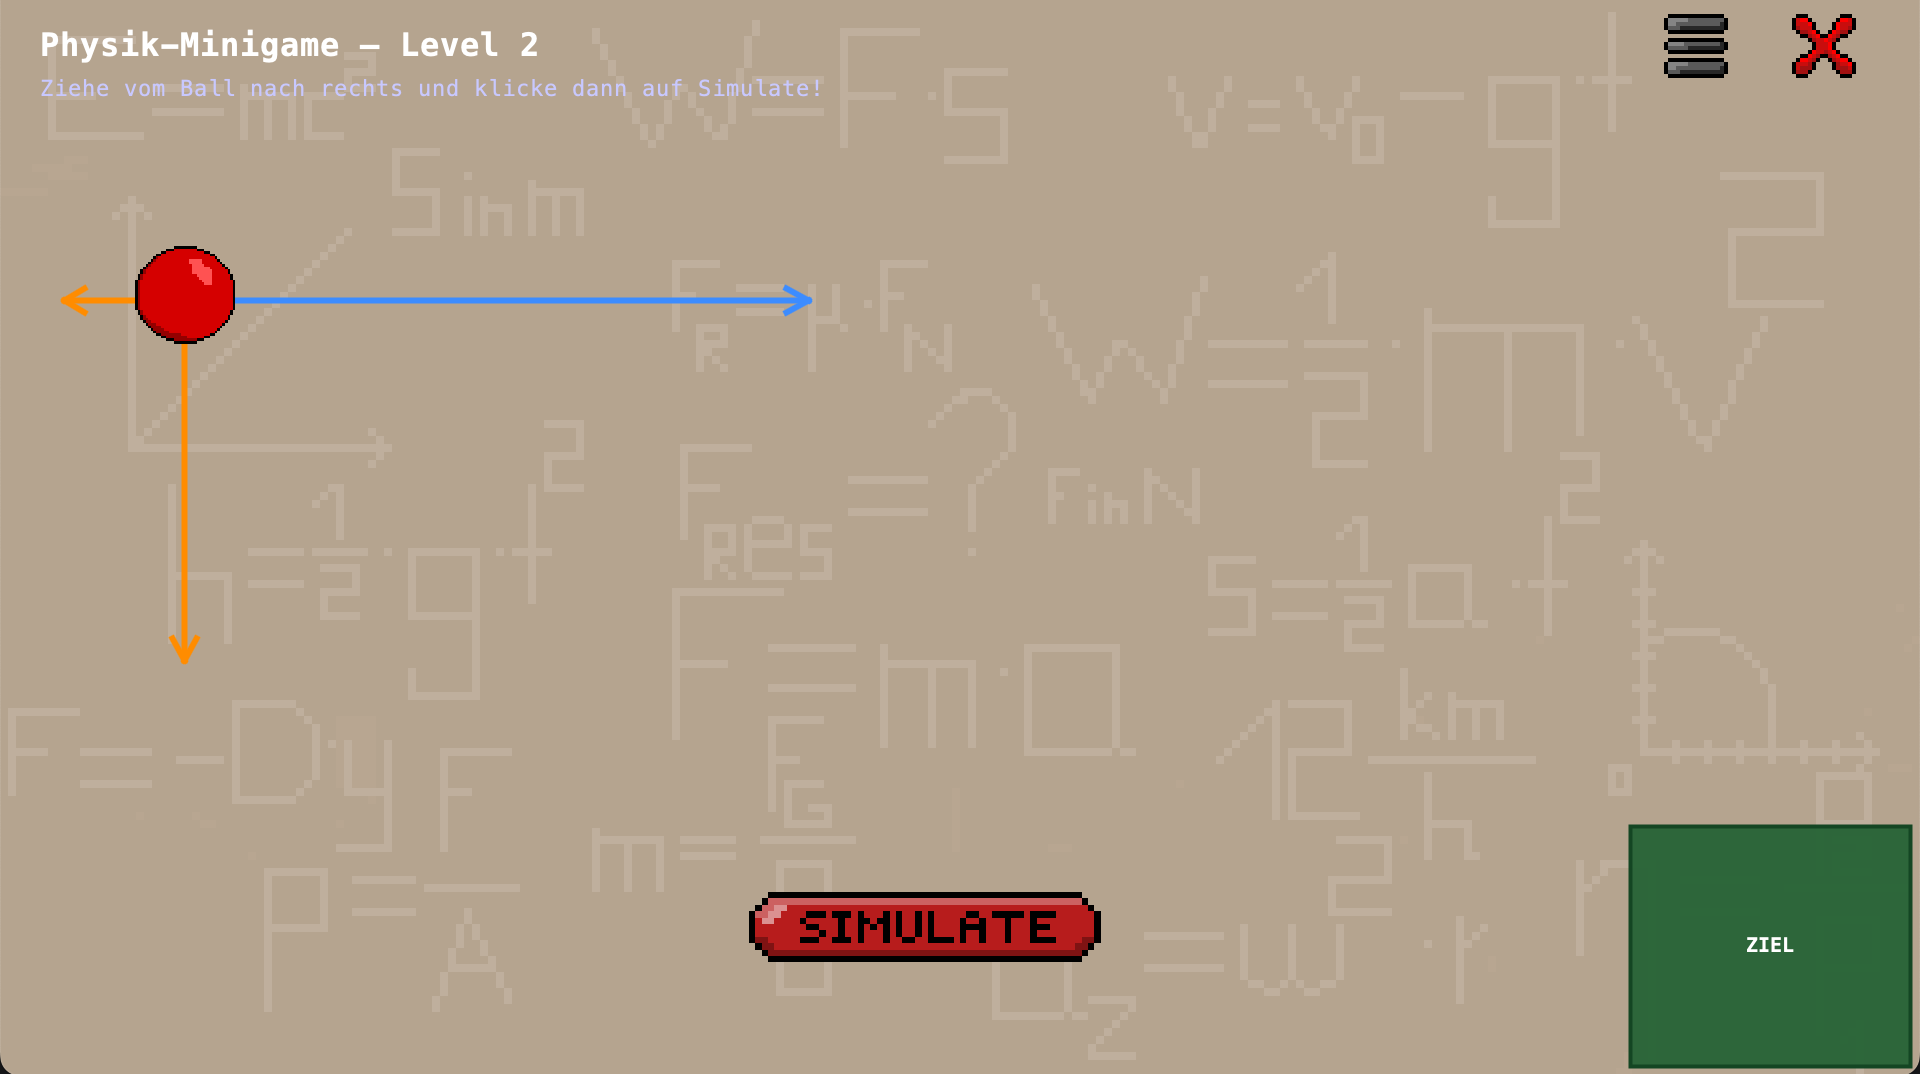
\includegraphics[width=\textwidth]{../dokumentation/bilder/BeispielPhysik.png}
			\caption{Beispiel Physik-Minigame}
		\end{figure}
	\end{minipage}
\end{frame}

\begin{frame}
	\frametitle{Spielmechanik}
      \begin{figure}
        \centering
        \begin{minipage}[l]{0.3\textwidth}
          \centering
          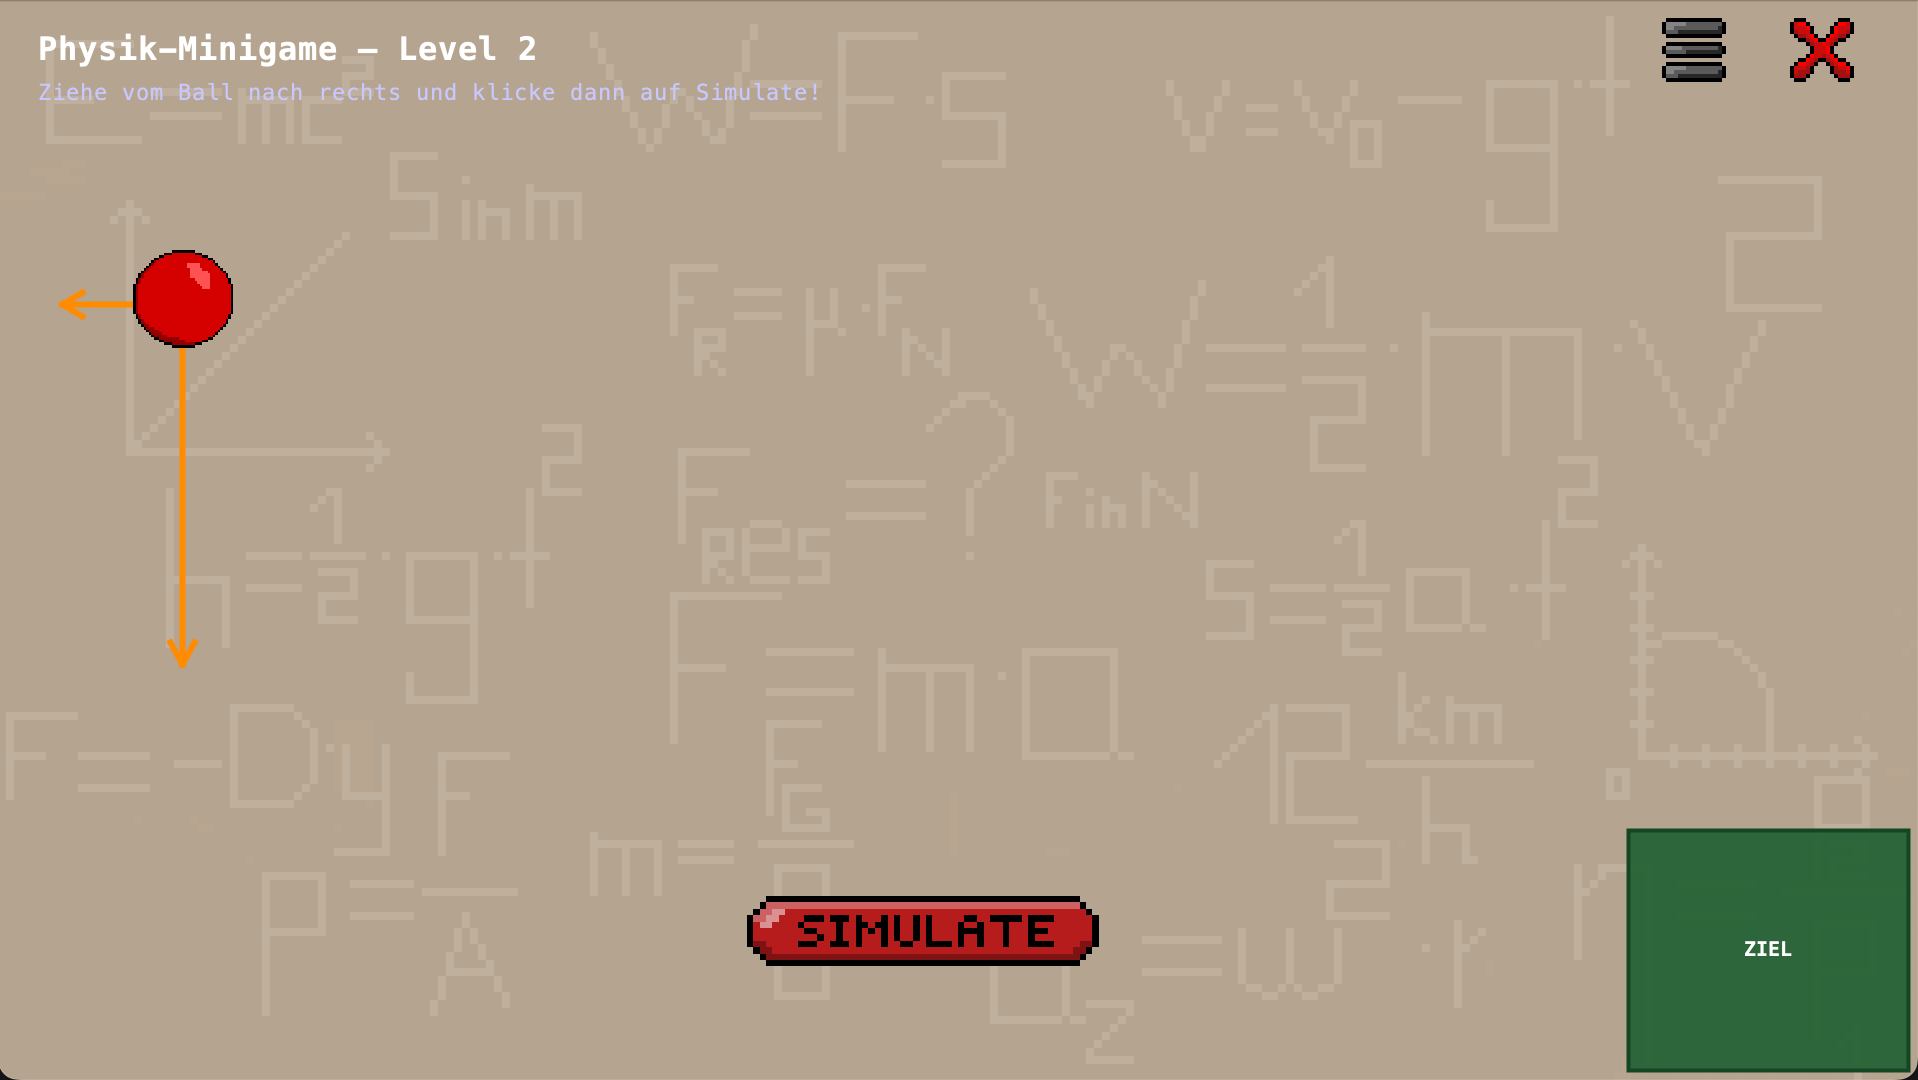
\includegraphics[width=\linewidth]{../präsi/bilder/PhysikLevelStart.png}
          \caption{Levelstart}
        \end{minipage}
        \hfill
        $\Rightarrow$
        \hfill
        \begin{minipage}[l]{0.3\textwidth}
          \centering
          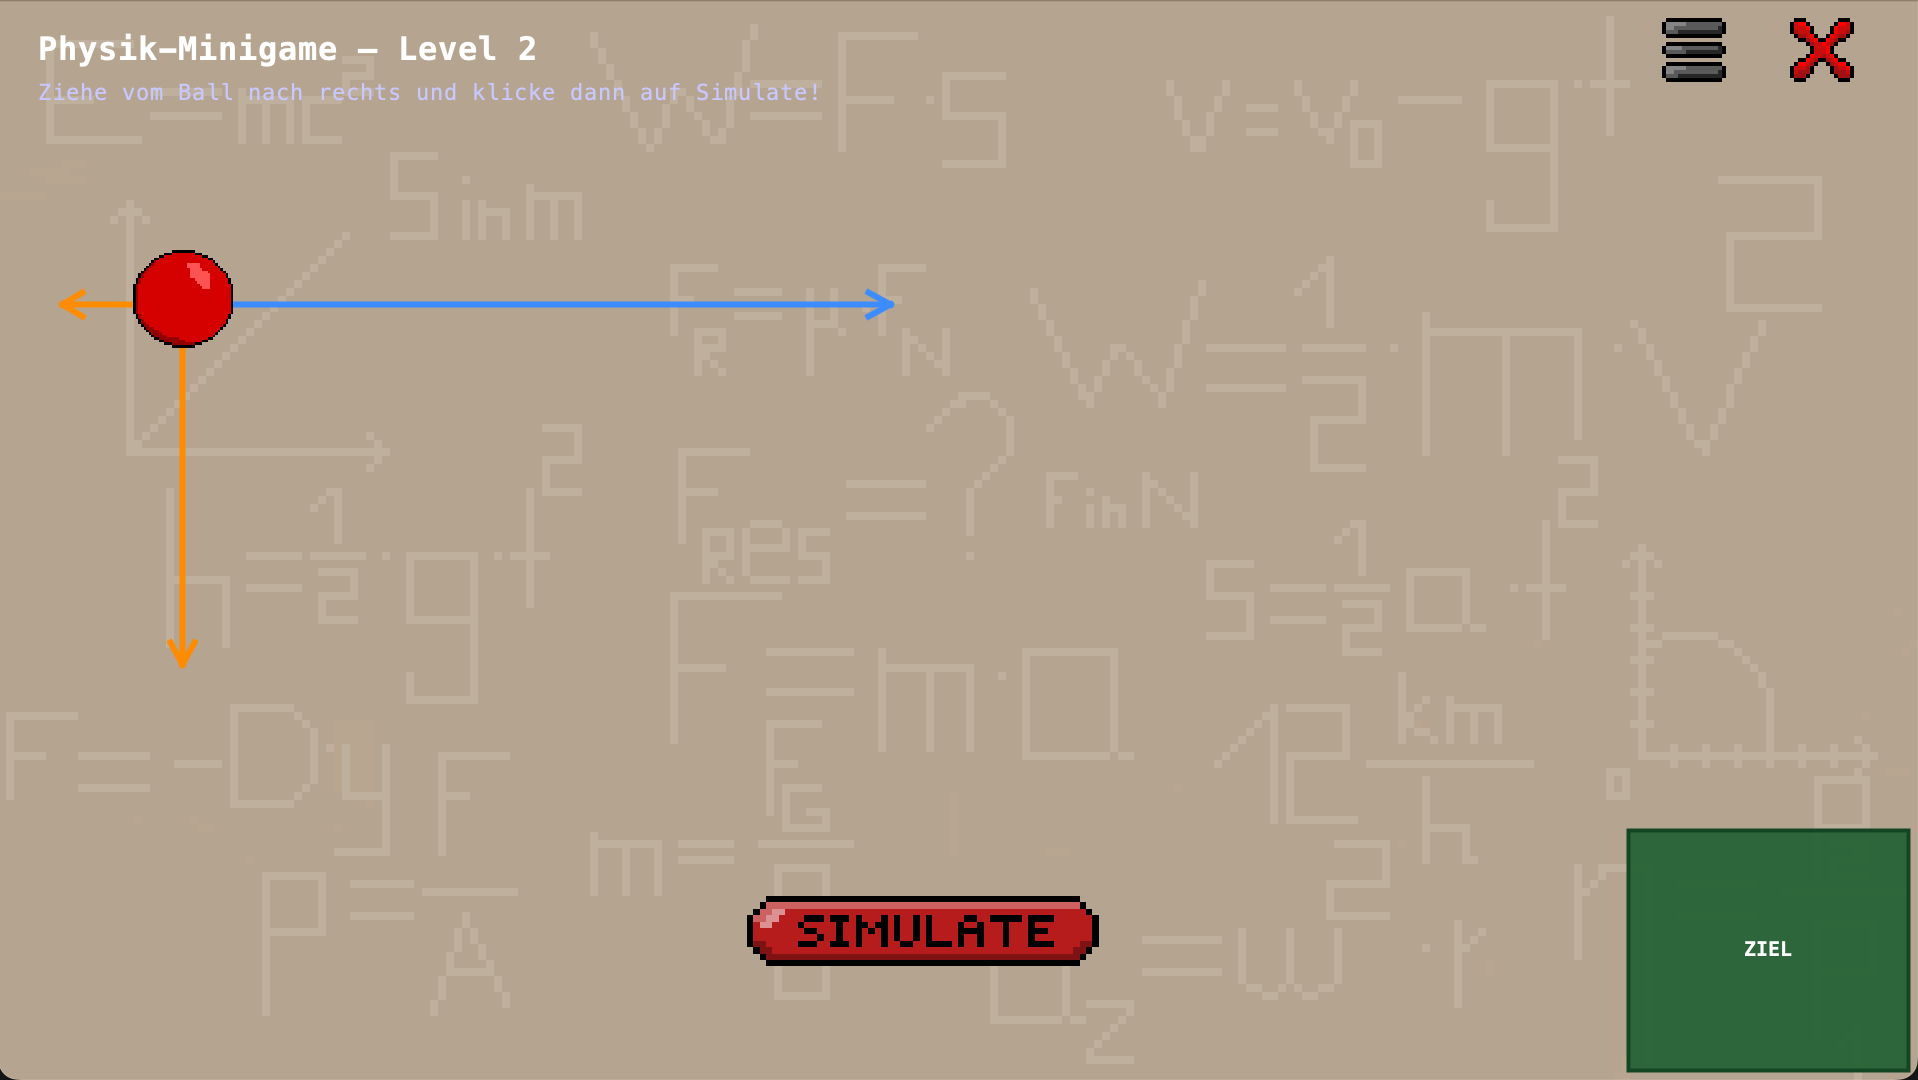
\includegraphics[width=\linewidth]{../präsi/bilder/PhysikSpielerkraft.png}
          \caption{Spielerkraft einstellen}
        \end{minipage}
        \hfill
        $\Rightarrow$
        \hfill
        \begin{minipage}[l]{0.3\textwidth}
          \centering
          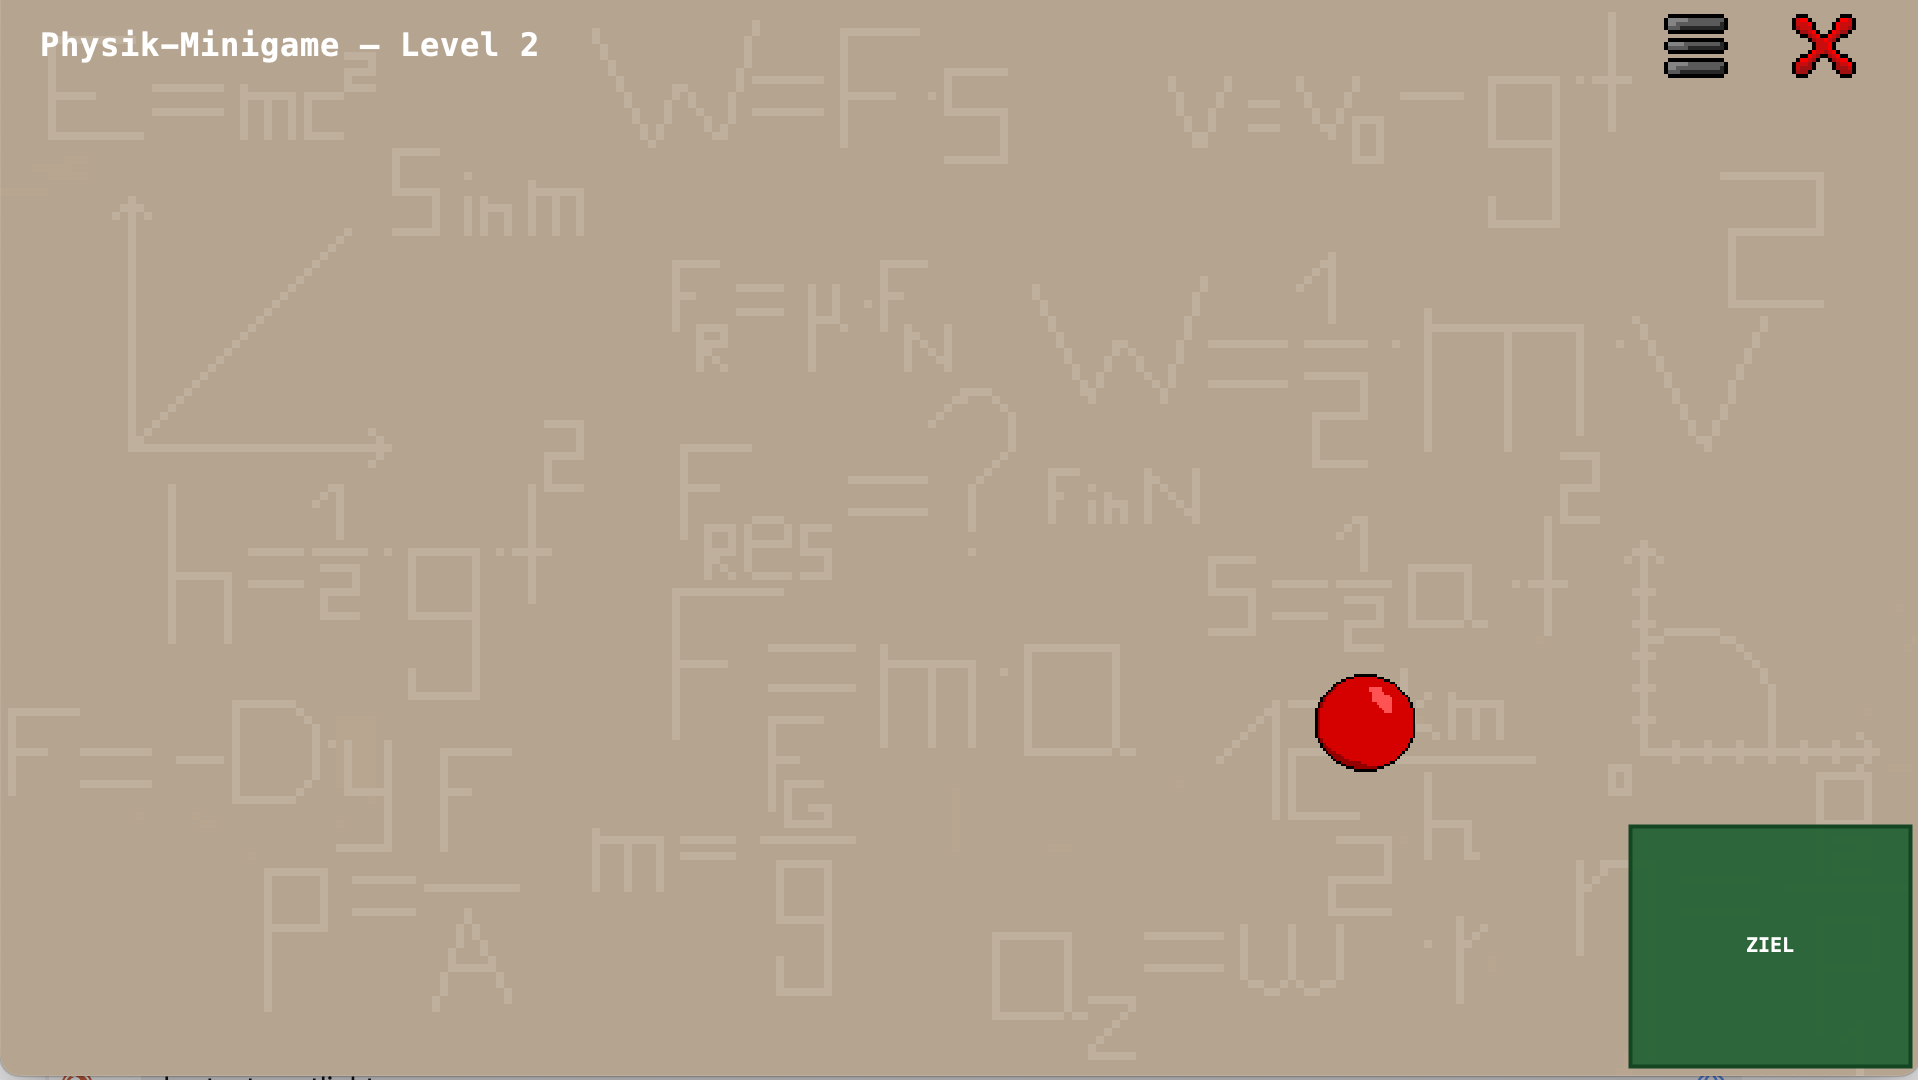
\includegraphics[width=\linewidth]{../präsi/bilder/PhysikFlug.png}
            \caption{Flugphase}
        \end{minipage}
      \end{figure}
\end{frame}


\begin{frame}
	\frametitle{PhysikLevelScene}

Sie beinhaltet:
	\begin{itemize}
		\item \texttt{reset()}
		\item \texttt{PhysikLevelScene(int level)}
	\end{itemize}
\end{frame}

\begin{frame}
	\frametitle{PhysikGameObject}

\begin{itemize}
        \item \textbf{Phase 1 – Vorbereitung}
        \begin{itemize}
            \item Basiskräfte levelspezifisch zeichnen
            \item Spieler*in zieht Kraftpfeil vom Ball weg (\texttt{kraftRichtung}
            \item Start: \texttt{simulateButton}
        \end{itemize} 
 \pause
        \item \textbf{Phase 2 – Simulation} 
        \begin{itemize} 
            \item \texttt{simulationStarten()}: Spielerkraft als Startgeschwindigkeit
            \item \texttt{ballBewegen()} wendet \texttt{basisBeschleunigungen} an
            \begin{itemize}
            	\item[$\Rightarrow$] prüft Kollisionen mit Rand, Wand, Ziel
            \end{itemize}
        \end{itemize}
 \pause
        \item \textbf{Phase 3 – Ergebnis} 
        \begin{itemize}
            \item \texttt{simulationStoppen(treffer)} -> \texttt{levelWon()}/\texttt{levelLost()}
            \item \texttt{draw()} zeigt Ergebnis; \texttt{levelInitialisieren()} setzt Level zurück
        \end{itemize}
    \end{itemize}
\end{frame}

\begin{frame}
	\frametitle{Das Biologie Minigame}
	\begin{minipage}[l]{0.40\textwidth}
		\begin{itemize}
			\item Konzept: Pflanzen- testat
			\item Level: schwierigere Pflanzen und überschüssige Label
		\end{itemize}
	\end{minipage}
	\begin{minipage}[r]{0.55\textwidth}
		\centering
		\begin{figure}
			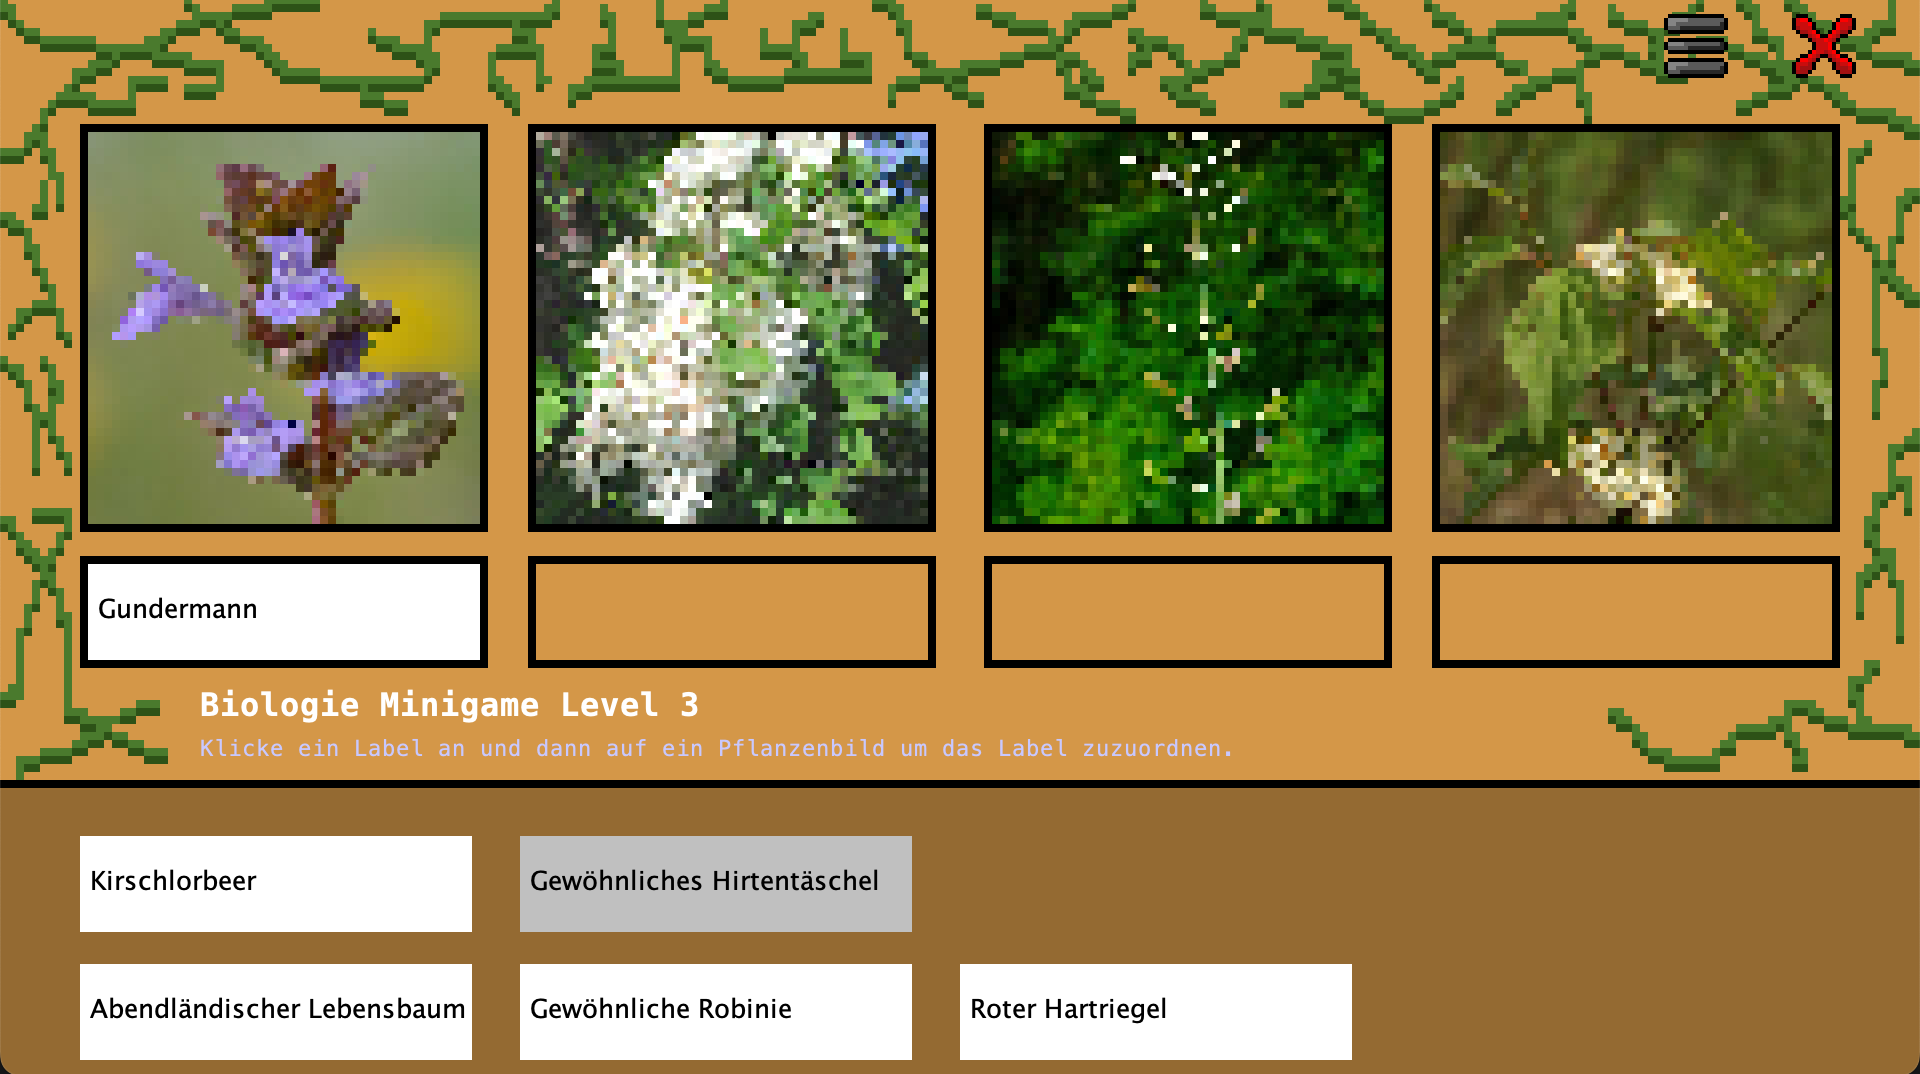
\includegraphics[width=\textwidth]{../dokumentation/bilder/BeispielBiologie.png}
			\caption{Beispiel Biologie-Minigame}
		\end{figure}
	\end{minipage}
\end{frame}


\begin{frame}
	\frametitle{BiologyData und BiologyPlant}
    \begin{itemize}
                \item BiologyData: Levelspezifische Arrays mit Pflanzenbildern
                \item BiologyPlant: einzelne Pflanze (Name und Bild)
            \end{itemize}
\end{frame}

\begin{frame}
	\frametitle{BiologyLevelScene}
\begin{itemize}
        \item \textbf{Spielaufbau}
        \begin{itemize} 
            \item 4 zufällig gewählte Pflanzen (\texttt{chosen})
            \item \texttt{reset()} neues Level mit neuen Pflanzen
        \end{itemize}
         \pause
        \item \textbf{Interaktion} 
        \begin{itemize} 
            \item \texttt{update()} verarbeitet Klicks: Label auswählen, abwählen\\
                  oder Bild zuordnen (\texttt{selectedLabel})
            \item \texttt{getLabelAtSlot(slot)} gibt aktuell platziertes Label zurück
        \end{itemize}
         \pause

        \item \textbf{Auswertung} 
        \begin{itemize}
            \item \texttt{allPlaced()} prüft, ob alle vier Slots belegt sind
            \item \texttt{checkWin()} vergleicht jedes Label mit  Pflanzennamen -> LevelWon/LevelLost
        \end{itemize}
    \end{itemize}
\end{frame}

\begin{frame}
	\frametitle{BiologyLabelObject}

Die Klasse beinhaltet:
	\begin{itemize}
		\item \texttt{name}
		\item \texttt{selected}
		\item \texttt{draw(Graphics2D g)}
	\end{itemize}
\end{frame}

